\section{Introduction}

Runtime verification (RV)  \cite{bartocci18,havelund-rv-data-2018} very generally refers to the use of rigorous (formal) 
techniques for {\em processing} execution traces emitted by a system being observed. The purpose is typically
%, again generally viewed, 
to evaluate the state of the observed system. Processing can take numerous
forms. We focus here on {\em specification-based} runtime verification, where an execution trace is checked against a property expressed in a formal logic, in our case variants of linear temporal logic.

Linear Temporal Logic (LTL) is a common specification formalism for reactive and concurrent systems. It is often used in e.g. model checking and runtime verification. Another formalism that is used for the same purpose is finite automata, often over infinite words. This includes B\"{u}chi, Rabin, Street, Muller and Parity automata~\cite{Thomas}, all having the same expressive power. In fact, model checking of an LTL specification
is usually performed by first translating the specification into a B\"{u}chi automaton. The automata formalisms are more expressive than LTL, with a classical example By Wolper~\cite{Wolper} showing that
it is not possible to express in LTL that every even state in
the sequence satisfies $p$. This has motivated extending LTL
in various ways.
We are mainly motivated by runtime verification of executions {\em with data}, for which a first-order temporal logic is
appropriate. There, too, we show that expressiveness can be extended.

We present first an extension of  propositional LTL that is based on using additional (auxiliary) propositions, not appearing in the execution, which are dependent on the past 
of the current execution. These propositions obtain their value in a state as a function of the prefix of the execution up and including that state through a past temporal formula. This can be seen as adding
summary states to the temporal specification, resulting in a specification that is in between logic and finite automata representation. This extension, which we believe is conceptually simpler
and more intuitive than other suggested extensions, is shown to be
equivalent to the other common specification formalism:
B\"{u}chi automata, regular expressions and quantified LTL.

We then proceed to first-order LTL. We relativise Wolper's example to the first
order case to motivate the need for
extending first-order LTL. Another example is based on the unexpressiveness of the transitive closure of a relation in first order logic, where, e.g., using a relation representing neighbors in a graph is not enough for representing that there is a path between nodes.
We present an extension where auxiliary relations, not appearing in the execution, are
added. While this extension
is capable of expressing the above
properties, we show that for the first-order version, this has less 
expressive power than adding full quantification over relations. This in distinction from adding quantification to propositional LTL, where prefixing existential quantification
provides the full expressive power of, say, B\"{u}chi automata.

The extensions we proposed to the logics are in particular natural for
runtime verification of past (safety) temporal properties, since
the values of propositional and first-order LTL are based
on calculating and updating a summary of the prefix of the execution. Runtime verification is often restricted to a {\em past}  version of temporal logic~\cite{HR}, mainly because for past properties we can decide when the monitored property is violated after monitoring a finite prefix of it, while for future properties we may never know for sure. Consistent with that, 
we provide runtime verification algorithms for the past-time versions of the extended propositional and first-order
logics. We further present an extension of the 
\dejavu{} tool (publicly available on {\sf github},
hidden here because of anonymous reviewing)
\ignore{(https://github.com/havelund/dejavu)} that
realizes the extended first-order past temporal logic verification. The \dejavu{} tool~\cite{HPU,HP} allows runtime verification on past time first-order temporal logic over infinite domains (e.g., the integers, strings). It achieves efficiency by using BDD representation of enumerations of data, rather than over the data values themselves, and by using
a garbage collection algorithm. 

The contributions of this paper are both theoretical and practical. On the theory side, we present and study extensions for propositional and first order linear-temporal logics and show the relations between them and existing versions. 
On the practical side, we present RV algorithms for the extended logic, and 
show how to cast them specifically in an efficient BDD-based implementation. We present some experiments performed with our implementation and report on the results. 

The structure of this paper is as follows. In Section~2 we first define the syntax and semantics of propositional temporal logic. We then review some of its classical extensions and present our own extension. In Section~3 we present a runtime verification algorithm for the extended past LTL. In Section~4 we review first order linear temporal logic, present our extension and study the relationships between the presented versions of first-order LTL. In Section~5 we present a runtime verification algorithm for the past version of the extended first-order LTL. Section~6 describes the implementation and provides experimental results. Finally, Section~7 concludes the paper.

%\klaus{I think that the structure of the paper should be
%crystal clear so that the reader does not get lost. A lost reader leads to rejection. If a reader understand the structure, but perhaps not the details, the reader may still be happy.}

\vspace{1ex}
\noindent {\bf Related work.}
For propositional LTL, the logic ETL~\cite{Wolper,WVS} extends
the set of temporal operators 
by using automata (or, equivalently a right linear grammar). Each automaton defines a temporal operator, where the input letters of that automaton correspond to future temporal subformulas. Each accepted run of such an automaton defines then the places
where the subformulas need to hold. Another expressive-equivalent extension, 
in~\cite{Wolper}, adds dynamic, i.e.,
state-dependent, quantification over propositions to LTL.

Addition of relations to temporal databases is done
for aggregation~\cite{Libkin}, where relations are
calculated, based on the current state, and are used for further calculating
functions (sums, maxima) over the sequence of states. Aggregations were also used in the runtime verification tool 
{\sf MonPoly}~\cite{agrebasin}.
%
% --- other less directly related work: ---
%
Numerous other systems have been produced for monitoring
execution traces eith data against formal specifications. 
These include e.g. \cite{LOLA,larva,halle-beepbeep-ieee-12,Meredith2011,Reger2015}. 

% ----------------

\iffalse
The contributions of the papers are both theoretical, and
practical. We study the extensions of propositional temporal logic (both full version and past/safety version) and suggest a restricted (and, to our opinion, an intuitive) extension that is equivalent to the power of quantified LTL or B\"{u}chi/finite automata. We then study 
The corresponding extension to first-order LTL, replacing propositions with relations, and allowing variables and constant values. We propose, for the first-order version, an extension similar to the one we propose for the propositional case. But then we show that for the first-order case, this extension has
less expressive power than adding quantification in the style of propositional temporal logic.

The extensions we suggest are in particular easy to implement, as an extension to existing propositional/first-order runtime verification. We extend our tool \dejavu, experiment with new examples that take advantage of the extension.
\fi
\vspace{1ex}
\noindent {\bf Conventions.}
\label{sec:prelim}
In this paper, we treat and present several versions of the logic LTL. To simplify
the presentation, we prefix LTL with letters as follows:

\begin{itemize}
\item{P} restricts to P{\em ast} temporal operators.
\item{F} allows F{\em irst-order} quantification over
data assigned to variables that is uniform for all states. This quantification is referred to as {\em static} quantification.
\item{Q} adds (second-order) Q{\em uantification} that is state-dependent. This is referred to as {\em dynamic} quantification.
\item{E} allows E{\em xtending} the 
set of objects that occur in the input with
new auxiliary predicates (for the propositional versions) or relations (for the first-order cases) using past temporal logic rules that define them.
\end{itemize}

%\klaus{You above introduce some concepts before they really are explained. Q and E. I understand why you do this (to have it in one place), but it may be too difficult for the reader to grasp if not "initiated".
%Especially the E.}

%\klaus{We use ELTL (etc) to denote Extended LTL. 
%But QLTL is also an extension of LTL. These logics 
%are all extensions of LTL. Perhaps RLTL (for Rule-based 
%LTL) would have been better ... or something. Not urgent, 
%we can always change that if we want to.}

%\klaus{The explanation of Q and E could be improved.}


%\doron{Did my best to make the letters more self explained. I think R is usually reserved in temporal logic for realtime. But if you insist, one thing that I cannot perform from here is changing the two figures where these letters occur.}


\newcommand\eventty{\mathbb{E}}
\newcommand\setof[1]{\mathcal{P}(#1)}


\section{Propositional LTL}
\label{propLTL}

The classical definition of linear temporal logic~\cite{MP} has the following syntax:
\[ \varphi ::= \true \, | \,  p \, | \, ( \varphi \wedge \varphi ) \, |  \, \neg  \varphi \, |   \, \bigcirc \varphi \, |  
\, ( \varphi  \until  \varphi ) \,|  \, \ominus \varphi |
   \, ( \varphi \ \since \ \psi ) \,  \]
where $p$ is a proposition from a finite set of propositions $P$, and $\bigcirc$, $\until$, $\ominus$, $\since$ stand for {\em next-time}, 
{\em until}, {\em previous-time} and {\em since}, respectively.


The models for LTL formulas 
are infinite sequence of states, of the form
$\sigma =  s_{1}\, s_{2}\, s_3 \ldots$,
where $s_i \subseteq P$ for each $i\geq 1$. These are the propositions that {\em hold} in that state.
%We denote by $\xi_{i}$ the suffix $s_{i} s_{i+1} s_{i+2}\ldots$ of $\sigma$. 
LTL's semantics is defined as follows:
\begin{itemize}
\item $( \sigma, {i}) \models \mathit{true}$.
\item $(\sigma, {i}) \models p$ iff $p \in s_{i}$.
\item $(\sigma, {i}) \models \neg\varphi$ iff  $(\sigma, {i}) \not\models \varphi$.
\item $(\sigma, {i}) \models ( \varphi \land \psi)$ iff $(\sigma, {i}) \models \varphi$ and $(\sigma, {i} ) \models \psi$.
\item $(\sigma, {i}) \models \bigcirc \varphi$ iff $(\sigma, {i+1}) \models \varphi$.
\item $(\sigma, {i}) \models ( \varphi  \cal{U}  \psi )$ iff for some $j$,
$j\geq i$, $(\sigma, {j}) \models \psi$,
and for each $k$, $i \leq k < j$, $(\sigma, {k}) \models \varphi$.
\item $(\sigma , i) \models \ominus \varphi$ iff $i > 1$ and $(\sigma, i-1) \models \varphi$.
\item $(\sigma , i) \models (\varphi \since \psi)$ iff there exists $j$, $1 \leq j \leq i$, such that
$(\sigma , j)  \models \psi$ and for each
$k$, $j < k \leq i$, $(\sigma , k ) \models \varphi$.
\end{itemize}
Then $\sigma \models \varphi$ when $( \sigma ,1 ) \models \varphi$.
We can use the following abbreviations:
$\false = \neg \true$, 
$(\varphi \vee \psi) = \neg ( \neg \varphi \wedge \neg \psi )$, 
$(\varphi \rightarrow \psi) = ( \neg \varphi \vee \psi)$,
$(\varphi \leftrightarrow \psi) = ((\neg \varphi \wedge \neg \psi) \vee (\varphi \wedge \psi ))$,
$\Diamond \varphi = (\true \until \varphi)$ and $\Box \varphi = \neg \Diamond \neg \varphi$,
${\bf P}\  \varphi = (\true \; \since \; \varphi)$ ({\bf P} stands for P{\em reviously}), and 
${\bf H}\  \varphi = \neg {\bf P}\ \neg \varphi$ ({\bf H} stands for 
H{\em istory}).



%%infinite sequences (finite executions can be extended by repeating the last event indefinitely to form an infinite paths).
The expressive power of different versions of propositional LTL is often compared to regular expressions
over the alphabet $\Sigma = 2^P$ and to  {\em monadic} first and second-order logics where the temporal propositions
correspond to unary predicates (over time). An overview appears in~\cite{Thomas}. Accordingly, we have the following characterizations:
LTL is equivalent to monadic first-order logic\footnote{First-order logic with unary predicates over the naturals, and the relation $<$.},  star-free regular expressions\footnote{Regular expressions but without star operator (or $\omega$).} and counter-free B\"{u}chi automata\footnote{A counter-free language is a regular language for which there is an integer $n$ such that for all words x, y, z and integers $m \geq n$ we have that $xy^m z \in L$ if and only if $xy^n z \in L$.}. In fact, restricting the temporal operators to the {\em future}  operators $\until$ and $\bigcirc$
(and the ones derived from them $\Box$ and $\Diamond$)
leaves the same expressive power and is commonly used. 

%\klaus{Is that also the true for the first-order case? Doron: I have no idea. But at this point, I would not ask to ask Gabbay.}

An important subset of LTL, called here PLTL, allows only past temporal
operators: $\since$, $\ominus$ and the operators derived
from them, $\mathbf{H}$ and $\mathbf{P}$. The past time logic is sometimes interpreted over finite sequences, 
where $\sigma \models \varphi$ when $( \sigma , | \sigma | ) \models \varphi$.
Alternatively,
it is also a common practice to use the past time restricted version, prefixed with  a single $\Box$ (always) operator; in this case, each of the prefixes has to satisfy $\varphi$. This later
form expresses {\em safety} LTL properties~\cite{AS} over infinite sequences. 
(When PLTL is interpreted over finite sequences, its
expressive power is the same as star-free regular expressions, first-order monadic logic over finite sequences and counting-free automata.)


%\section*{Extending Propositional LTL}
\label{sec:extending-prop-ltl}



Wolper~\cite{Wolper} showed that the expressive power of LTL is lacking with respect
to some important properties. As a canonical example, he demonstrated that it is impossible to
express that all the states with even indexes in a sequence
satisfy $p$ (this is
different than saying that $p$ alternates between $\true$ and $\false$ on consecutive states).
Wolper's example property cannot be expressed in PLTL either.
In order to extend the expressiveness of LTL, Wolper suggested to use linear grammars, or, alternatively, the ability to quantify over
propositions, as shown below.

\subsubsection{Extending LTL with dynamic quantification.}
Adding quantification over propositions, as done in~\cite{Wolper}, allows writing a formula of the form
$\Exists q \, \varphi$, where
$\Exists q$ represents {\em existential} quantification over a proposition $q$ that can appear in $\varphi$.

%A model for such a formula 
%has truth assignments only over the propositions in $B$, but the propositions $A$ can appear (only) within the scope of a quantifier.
To define the semantics, let $X \subseteq P$ 
%be a subset of 
%the propositional variables appearing in the %states of the sequence $\sigma = s_1 s_2 %\ldots$
and denote $\sigma |_X = s_1 \setminus X \, s_2 \setminus X \ldots$. (Note that $\sigma |_X$ denotes projecting {\em out} the variables in $X$.)



\begin{itemize}
\item $( \sigma, i ) \models \boldsymbol{\Exists} q \, \varphi$ iff there exists
$\sigma'$ such that $\sigma' |_{\{ q \} } = \sigma$ and 
$( \sigma', i) \models \varphi$.
\end{itemize}
%Since all the auxiliary variables appear in the scope of
%quantifiers, it holds that $\sigma \models \varphi$
%(in $\varphi$, auxiliary variables appear only within
%the scope of quantifiers)
%iff $\sigma |_A \models \varphi$.
%
%\klaus{Are the last two lines above needed?}
%
Universal quantification is also allowed, where $\Forall q\, \varphi =
\neg \Exists q\, \neg \varphi$.
This kind of quantification is considered to be {\em dynamic}, since the quantified variables can have different truth values depending on the states. It is also called  {\em second-order} quantification, since the quantification establishes the {\em set} of states in which a propositional variable has the value $\true$.
Extending LTL with such quantification, the logic QLTL has the same expressive power as regular expressions, full B\"{u}chi
automata, or monadic second-order logic with unary predicates over the naturals, see again~\cite{Thomas}.
In fact, it is sufficient to restrict the quantification to existential quantifiers that prefix the formula to obtain the full expressiveness of QLTL~\cite{Thomas}. 

Wolper's property can be expressed in QLTL as follows:
\begin{equation} \label{form0} \Exists q \,
( (  \neg q \wedge \Box (q \leftrightarrow \bigcirc \neg q )  )  \wedge \Box (q \rightarrow p ) )\end{equation}

Restricting QPLTL to the past modalities, one obtain the logic PQLTL. PQLTL has the same expressive
power as regular expressions and finite automata.
Equation~(\ref{form0}) can
be rewritten in PQLTL as:
\begin{equation} \label{form1} \Exists q \,
{\bf H} (( q \leftrightarrow \ominus \neg q )   \wedge (q \rightarrow p ) )\end{equation}
%In fact, it can be shown that a single existential quantifier is sufficient. 
Since $\ominus \varphi $ is interpreted as  $\false$ in the first state of any sequence, regardless of $\varphi$, then
$q$ is $\false$ in the first state. Then $q$ alternates between even and odd states.


%Note that since finite automata over finite sequences can be determinized, it is always sufficient to translate a
%PQLTL property into a deterministic
%automaton.


\subsubsection{Extending LTL with rules.}

We introduce now another extension of LTL, which we call ELTL.
%It has a form that puts it, conceptually, in between temporal
%logic and automata: on the one hand, it is possible to simply write
%a pure LTL formula, and on the other hand, one can write a specification that resembles a finite automaton. 
As will be showed later, this extension is
is very natural for runtime verification.

We partition the propositions $P$ into
{\em auxiliary propositions} $A = \{ a_1 , \; \ldots\; , a_n \}$
and {\em basic propositions} $B$.
%A model for an ELTL formula has truth assignments only over the propositions in $B$.
An ELTL property $\eta$ has the following form: 
\begin{equation} \label{ELTL}
\psi \mathit{\ where\ } a_j  := \varphi_j \, : \, 
 {j \in \{1, \ldots , n\}} \end{equation}
where each $a_j$ is a distinct auxiliary proposition from $A$,
$\psi$ is an LTL property and each $\varphi_i$ 
is a PLTL property where propositions from $B$ can
only occur within the scope of a $\ominus$ operator.
The semantics can be defined as follows. We refer to $\psi$
as the {\em statement} of $\eta$ and to 
$a_j  := \varphi_j$ as a {\em rule}. In text, rules
 will be separated from each other by commas. 
\begin{tabbing}
\ \ \ $\sigma \models \eta$ \=  if there exists $\sigma'$, where
$\sigma' |_A = \sigma$ such that \\
 \> $\sigma' \models ( \psi  \wedge   \Box \bigwedge_{1 \leq j \leq n} ( a_j \leftrightarrow \varphi_j)) $
\end{tabbing}

\noindent
Wolper's example can be written in ELTL
as follows:
\begin{equation} 
\label{form3}
\Box ( q \rightarrow p ) \, \mathrm{where} \, 
 ( q := \ominus \neg q)
\end{equation}
where $A = \{ q\}$ and $B = \{ p \}$.
The auxiliary variable $q$ is used to augment the input sequence such that each {\em odd} state will satisfy $\neg q$
and each {\em even} state will satisfy $p$.  


ELTL extends the set of propositional variables with new variables, whose values at a state are
functions of (i.e., uniquely defined by) the prefix of the model up to that state. The added propositions effectively summarize the past execution prefix up to and
including the current state.
This differs from 
the use of auxiliary variables in QLTL, where the values assigned to the
auxiliary variables do not have to extend the 
states of the model in a unique way throughout the interpretation of 
the property over a model. The constraint that auxiliary variables appearing in the formulas $\varphi_i$ 
must occur within the scope of a $\ominus$ operator
is required to help preventing that the values
of the auxiliary variables are conflicting, as in
$a_1 := \neg a_2$ and $a_2 := a_1$, which makes a formula
that uses $a_1$ and $a_2$ uniformly $\false$. Still, one can write unsatisfiable rules, e.g., by using the rule $a_1 : = \false$.

\begin{lemma} \label{fourone}
Let $\varphi$ be an ELTL formula
over the auxiliary propositions $A = \{ a_1 , \ldots , a_n \}$ and basic propositions $B$, with
a set of rules $a_j  := \varphi_j \, : \, 
 {j \in \{1, \ldots , n\}}$. 
Let $\sigma$ be a model with states over the $B$. 
Then there is at most one
model $\sigma'$ such that $\sigma' |_A = \sigma$ and $\sigma' \models \Box \bigwedge_{1 \leq j \leq n} ( a_j \leftrightarrow \varphi_j) $


\end{lemma}

%\klaus{(1) is this lemma saying the right thing? (2) is the proof really a proof of that lemma, (3) 
%$\varphi$s and the $\psi$s. Do we need a special greek symbol for it?}

\noindent {\bf Sketch of proof.} By induction on the state index. Each auxiliary variable
is defined, via a PLTL formula by the current state of the model over the values of the propositions $B$, and by the values of $A \cup B$ in previous states.  \qed
%A PLTL property depends in a state only on the prefix of the model that precedes and includes that state. 


\begin{theorem}
\label{theo1}
The expressive power of 
ELTL is the same as QLTL.
\end{theorem}
\noindent {\bf Proof.}
Each ELTL formula $\eta$, as defined above,
is expressible using the following equivalent QLTL formula:

\[   \Exists a_1 \ldots \Exists a_n  ( \psi  \wedge   \Box \bigwedge_{1 \leq j \leq n} ( a_j \leftrightarrow \varphi_j))
\]

%\klaus{How do we know that the ``other direction'' below is possible?}

\noindent
For the other direction, one can translate the QLTL property first into
a second-order monadic logic formula, then to a deterministic Muller automata and then construct an ELTL formula that holds for the accepting executions of this automaton. The rules of this formula encode the automata states, and the statement describes the acceptance condition of the Muller automaton.
The details of the
constructions are given in the appendix. \qed

%EPLTL, where the Muller automaton can be
%replaced with a B\"{u}chi automaton,
%where all of its states, except one, sink
%state, are accepting. \qed

\iffalse
The use of the auxiliary variables $a_1 \ldots a_n$ and the
rules of an ELTL specification 
can be viewed as representing a
state machine, in particular when the only modality that is used in the rules part is $\ominus$.
In that case, we can consider an ELTL specification $\eta$ as consisting of two synchronous parts: an LTL property 
(the statement) 
and a finite automaton, whose states correspond to combinations
of truth values of the auxiliary variables, and can be referred to
within $\psi$. As a corollary of Theorem~\ref{theo1}, 
this restricted representation is also equivalent to QLTL.
This representation can be useful, for RV, as explored further in this paper, because of the possibility to
incrementally calculate the values of the auxiliary variables. 
Similarly, it can be
used for extending the expressiveness of LTL model checking.


%\klaus{First sentence below sounds wrong: (1) PLTL already does not have future time operators, and (2) why mention infinite sequences?}
\fi

We define EPLTL by disallowing the future temporal operators (except an implied prefixing $\Box$) in ELTL. This results in
a formalism that is equivalent to finite (B\"{u}chi) automata, where all the states except one are accepting and where the non-accepting state is a sink. 
We can use a related, but simpler construction than in Theorem~\ref{theo1} to prove the following:


\iffalse
In this case, 
we replace the first part of the construction in the proof of Theorem~\ref{theo1}
with the simpler formula $\vee_{s \in A} a_s$, where all the states but one are
accepting.$A$ are the accepting states of the finite automaton.

\klaus{Last sentence above: perhaps say with words that we are always in an acceptance state - if that's what the point is.}
\fi

%For representing safety properties that can be expressed in QPLTL, we can use a restricted version as shown in the following simple Lemma.


\begin{lemma}
\label{simplecase}
The expressive power of 
EPLTL is the same as QPLTL.
%Any safety QPLTL property can be expressed using the following restricted
%ELTL form:
%\[  \Box p {\ where\ } a_j  = \varphi_j \, : \, 
% {j \in \{1, \ldots , n\}}  \] 
% with $p$ being one of the auxiliary variables %$a_j$.
\end{lemma}
In fact, it is easy to show that EPLTL can be restricted to the following form, while retaining its expressive power.
\[  \Box p {\ where\ } a_j  = \varphi_j \, : \, 
{j \in \{1, \ldots , n\}}  \] 
with $p$ being one of the auxiliary variables $a_j$. Yet, this may not be the preferred form
of an EPLTL property, and the use of further past-time temporal operators, and a non trivial statement  part may provide a more intuitive specification.
The relative expressive power between the propositional temporal logics discussed in this section is summarized in Figure~\ref{prop}. An arrow from A to B means that logic  B is more expressive than A. A double headed arrow shows same expressiveness

\iffalse
\noindent {\bf Proof.} The proof of the Lemma follows from the
axiomatization of QLTL in~\cite{MP}, e.g.,
$\varphi\ \since\ \psi \leftrightarrow \psi \vee ( \varphi \wedge (\varphi\ \since\ \psi))$. \qed

\klaus{In the axiom above, isn't there missing a $\ominus$ before
the second $(\varphi\ \since\ \psi)$?}

\klaus{Above: is the following really correct?: 
``with $p$ being one of the auxiliary variables $a_j$''.}

While this Lemma makes the use of the temporal operators
besides $\ominus$ in EPLTL redundant, it is still
convenient to use a combination of
temporal operators when possible, and
auxiliary variables definitions.
\fi








\begin{figure}
\begin{center}
%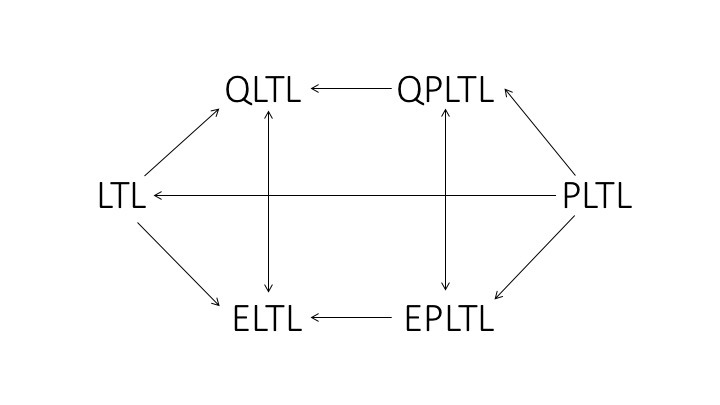
\includegraphics[height=0.6in,width=2in]{PROP.jpg}
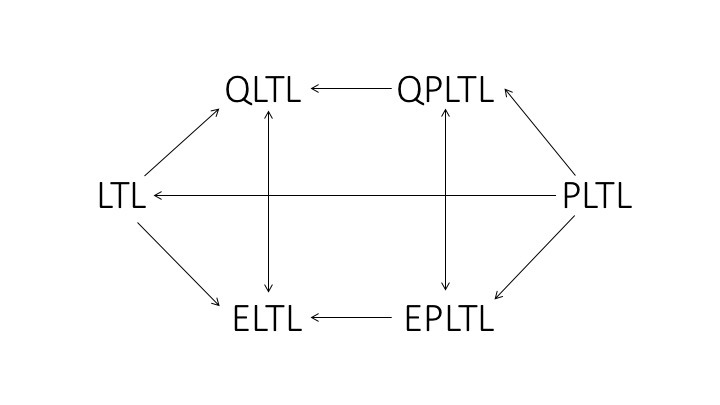
\includegraphics[width=2.8in]{PROP.jpg}
\caption{\label{prop}
Comparing the expressive power of the temporal logics in Section~\ref{propLTL}
}
\end{center}
\end{figure}




\section{RV for Propositional Past-Time LTL and its Extension}
\label{LTLruntime}

Runtime verification of temporal specifications often
concentrates on the past portion of the logic.  Past-time  specifications have the important property that one can distinguish when they are violated after observing a finite prefix of
an execution. For an extended discussion of this issue of {\em monitorability}, see e.g.,~\cite{Ugly,FFM}.

The algorithm for PLTL first presented in \cite{HR} 
is based on the observation that the semantics of the 
past time formulas $\ominus \varphi$ and $(\varphi\, \since \,\psi)$ in the current step $i$ is defined in terms of the semantics
in the previous step $i - 1$ of a subformula.
To demonstrate this, we repeat here the definition of the previous-time
operator $\ominus$, and rewrite the definition
of $\since$ in an equivalent form that is
more directly applicable for runtime verification.
\begin{itemize}
\item $( \sigma , i) \models \ominus \varphi$ iff $i > 1$ and $(\sigma, i-1) \models \varphi$.
\item $(\sigma , i) \models (\varphi \, \since \, \psi)$ iff $(\sigma , i) \models \psi$ or the following hold: $i>1$,
$( \sigma , i)  \models \varphi$ and 
$(\sigma , i-1 ) \models ( \varphi \, \since \, \psi )$.
\end{itemize}
Runtime verification for a PLTL formula $\eta$ exploits the fact that
the semantic definition is recursive in both the structure of the property. Thus, subformulas
are evaluated based on smaller subformulas, and the
evaluation of subformulas in the previous state.
The algorithm, shown below, uses two vectors (arrays) of values indexed by subformulas:  $\old$, which summarizes the truth values of the
subformulas for the execution prefix that
ends just {\em before} the new state, and $\current$, for the execution prefix that
ends with the {\em current} state. The order of calculating $\current$ for subformulas is bottom up, according to the syntax tree.
\begin{enumerate}
\item Initially, for each subformula $\varphi$
of $\eta$,
%$B ( \varphi , \current ) = \bfalse $.
$\current ( \varphi ) := \false$.

\item Observe a new event (as a set propositions) $s$ as input. 
\item Let $\old := \current$.
\item Make the following updates for each subformula. If $\varphi$ is
      a subformula of $\psi$ then $\current ( \varphi )$ is updated before 
      $\current ( \psi )$.
\begin{itemize}
  \item $\current ( \true ) := \true$.
  \item $\current (  \varphi \wedge \psi  ) := 
  \current ( \varphi )\  and\ \current ( \psi )$.
  \item $\current ( \neg \varphi  ) := not\ \current ( \varphi )$.
  \item $\current (  \varphi \since \psi  ) :=  
  \current ( \psi  )\ or\ ( \current ( \varphi ) \ and\ 
      \old ( ( \varphi \since  \psi )))$.
%DAP: I removed the \; around \since, since it penetrated the 2nd column!
  \item $\current ( \ominus \; \varphi ) := \old ( \varphi )$.
\end{itemize}
\item If $\current (\eta) = \false$ then
report a violation, otherwise goto step~2.
\end{enumerate}

\subsubsection*{Runtime verification for QPLTL.}  This can be performed by translating a
formula into a deterministic finite automaton, where one distinguished states, $s$, in a sink state.
Then the sequence of states to be checked forms the input for this automaton, and violation is
announced if $s$ is reached.
QPLTL can be extremely compact, in particular when using alternating existential and universal 
quantifiers, which can result in a huge (non-elementary) explosion of
the automaton representing the same
specification~\cite{Thomas}.


\subsubsection*{Runtime verification for EPLTL.} For EPLTL,  we need to  add to the above
algorithm calculations 
of $\current ( a_j )$ and
$\current ( \varphi_j )$, for each of the rules of
the form $a_j := \varphi_j$ (the corresponding
$\old$ entries will be updated as in line~3 in the above algorithm).

%(calculations
%for the statement part $\psi$ remain the same).
%$\current ( a_j )$ and $\old ( a_j )$,
%and perform the following between steps~3 and~4 %for each $a_j$: $\current ( a_j ) := \current ( %\varphi_j )$.

%For PLTL, we can calculate  $\current$, for subformulas,
%bottom up. But
Because the
auxiliary variables can appear recursively in EPLTL rules, the order of calculation is
subtle. To see this, consider, for example, the formula~(\ref{form3}). It contains
the definition $q := \ominus \neg q$. Now, we cannot calculate this
bottom up, as we did for PLTL, since $\current ( q )$ is not computed yet, and we need 
to calculate $\current ( \ominus \neg q )$ in order 
to compute $\current ( q )$.
However, notice that the calculation is not dependent on the
value of $q$ to calculate $\ominus \neg q$; 
in Step~4 above, we have that
$\current ( \ominus \; \varphi ) := \old ( \varphi )$
so  $\current ( \ominus \neg q ) := \old ( \neg q )$.

%\klaus{I don't see that we need to talk about the top-down evaluation.}

Under {\em mixed evaluation order}, one calculates $\current$ as part of Step~4 of the above algorithm in the following order. The first~four steps, $a$-$d$, are for the rules, and the fifth step $e$ is for the statement $\eta$.
\begin{description}
\item{\em a.} Calculate 
$\current ( \delta )$ for each subformula $\delta$
that appears in $\varphi_j$ of a rule
$a_j := \varphi_j$, but {\em not} within the scope of
a $\ominus$ operator. (This is not
a problem, since
$\current ( \ominus \gamma )$ is set to $\old ( \gamma )$.)
\item{\em b.} Set 
$\current ( a_j )$ to $\current ( \varphi_j )$ for each $j$.
\item{\em c.} Calculate $\current ( \delta )$ for each subformula $\delta$
that appears in $\varphi_j$ of a rule
$a_j := \varphi_j$ {\em  within} the scope of
a $\ominus$ operator.
\item{\em d.} Calculate $\current ( \delta )$ for each subformula $\delta$
that appears in the statement $\psi$, using the calculated $\current ( a_j )$.
\item{\em e.} Calculate $\current ( \eta )$ for the statement
$\eta$.
\end{description}



\section{First-Order LTL}

%section*{Syntax and Semantics}
\label{sec:syntax-semantics}

Assume a finite set of infinite domains\footnote{Finite domains are handled with some minor changes, see~\cite{HPU}.}
$D_1, D_2, \ldots$,
e.g., integers or strings. 
Let $V$ be a finite set of {\em variables}, 
with typical instances $x$, $y$, $z$.
%We denote by $x: D$ the fact that the variable $x$ has the domain $D$.
An {\em assignment} over a set of variables $V$
maps each variable $x \in V$ to a value from
its associated domain $\domain ( x )$, where multiple variables (or all of them)
can be related to the same domain. For example
$[ x \rightarrow 5 , y \rightarrow \text{``abc''} ]$ assigns
the values $5$ to $x$ and the value ``abc'' to $y$.
%Let ${\cal R}$ be a set of {\em relations} 
%with typical instances $R$.
%Each relation is associated with some position-dependent domains.

%\klaus{Above: let T be ... Is T used later? The relations are used in the next paragraph, why not introduce them there? Also, relations are not defined really.}
%\klaus{I don't quite understand the motivation below for this way of modeling events: relations with a time stamp, and the whole story of the time stamp not being mentioned etc. Why not just the usual models: traces? Too late to change now for CAV though.}

We define models for FLTL based on {\em temporal} relations~\cite{Chomicki}. That is relations with
last parameter
that is a natural number represented a time instance. So a tuple of
a relation $R$ can be $(``a", 5, ``cbb", 3)$, where
the  value $3$ is the time parameter. The last parameter $i$
does not correspond to modeling physical time. This
is rather used to allow the relations to have
different tuples in different instances of $i$,
corresponding to states, in the propositional temporal
logics.

For a relation $R$, $R [ i ]$ is the relation obtained from $R$ by
restricting it to the value $i$ in the last parameter, and removing that last $i$ from the tuples. For simplicity, we will describe henceforth
the logic with relations $R$ that have exactly two parameters, 
hence $R [ i ]$ will have just one parameter whose domain will be denoted as $d ( R )$. The definition of the logic over other numbers of parameters is quite straightforward. e.g., when $R$ has one parameter, $i$,
$R [ i ]$ is a Boolean value. Our implementation of runtime verification described later fully supports relations with zero or more parameter. This also applies to the extensions of the logic in the rest of this section, and to some of the examples used.

%\klaus{Above, what about instead of writing: ``this domain is fixed over all the values of the second parameter $i$'' to write:
%``this domain is independent of the values of the second %parameter $i$'' - if that is what you mean to say.}

%\klaus{Above: we need to say explicitly what $i$ intuitively is meant to represent: positions, time, ....}

\subsubsection{Syntax.} 

The formulas of the core FLTL logic are 
defined by the following grammar,where $p$ denotes a relation,
$a$ denotes a constant and $x$ denotes a variable. 
\begin{center}
$\varphi ::= \true  \; | \;
    p ( a ) \; | \;
    p ( x ) \; | \;
    ( \varphi \wedge \varphi ) \;  |   \;
   \neg \varphi \; | \;
   \bigcirc \varphi \; | \; 
   ( \varphi \; \until \; \varphi ) \; | $ %\\
   $ \ominus \; \varphi \; | \;
    ( \varphi  \; \since  \; \varphi ) \; | \;
    \exists x \; \varphi$
\end{center}

%We interpret a predicate $p(a)$ as a subformula that
%represents the occurrence of some
%For example, if we open
%a file named $\text{``xyz''}$, we may have $\mathit{open}
%(\text{``xyz''})$, where the
%domain of the predicate ${\mathit{open}}$ is over strings representing
%file names.

\noindent 
Additional operators are defined as in the propositional logic. We define
$\forall x \; \varphi = \neg \exists x \neg \varphi$.
Restricting the modal operators to the past operators
($\since$, $\ominus$ and the ones derived from them) 
forms the logic PFLTL.

\subsubsection*{Semantics.}
A model is a set of temporal
 relations ${\cal R} = \{ R_1 \, \ldots , R_m \}$.
 Since the standard definition of temporal logic is
 over a sequence (``the execution''), let
 ${\cal R} [ i ] = \{ R_1 [ i ] \, \ldots , R_m [ i ] \}$. ${\cal R} [i]$ represents a {\em state}.
 A model ${\cal R}$ can thus be seen as a sequence
 of states ${\cal R}[1] {\cal R}[2] \ldots$. Let 
 $m$ be a bijection
from relation names (syntax)
onto the relations ${\cal R}$ (semantics).
%After the formal semantical definition, we will abuse notation
%and use the same symbol for the representation of the relation in the logic and for the relation as mathematical object.

%\klaus{Above, did you not already say the following before:
%``we denote by $R_k [ i ]$ the restriction of
% the relation $R_k$ to the value $i$ of the last parameter.''.}

\iffalse
At a given state the formula
$p(\text{``a''})$ means that $p (\text{``a''} )$ holds
in the current state,
that is, $p (\text{``a''} )$ is among 
the ground predicates of the state.
Consider now the formula $p ( x )$, for a variable $x \in V$.
We interpret it such that $x$ is assigned any value ``$a$'' where
$p ( \text{``a''} )$ appears in the current state. 
%DP: Added parentheses on the outside level.
Thus, for interpreting $(p ( x ) \wedge q ( y ))$ in a state that
has the predicates
$p ( \text{``a''} )$ and $q ( 3 )$,
we have the assignment $[ x \mapsto \text{``a''} , y \mapsto 3 ]$.
%The past time temporal operators have the following intuitive meaning.
The formula $(\varphi_1\; \since\; \varphi_2)$ 
(reads $\varphi_1$ {\em since} $\varphi_2$)
means that $\varphi_2$ occurred in the past (including now)
and since then (beyond that state) $\varphi_1$ has been true. This is the 
past dual of the commonly used %DP: changed "common" to "commonly used".
future time  {\em until} modality~\cite{MP}. 
The property $\ominus \; \varphi$ means that $\varphi$ is true 
in the previous state.
This is the past dual of the %DP: removed "common".
future time {\em next} modality.
We can also define the following additional temporal operators:
$P \; \varphi = (\true \, \since \, \varphi)$ (``previously''),
and $H \varphi = \neg P \neg \varphi$ (``always in the past'' or ``historically'').
The operator $[\varphi_1,\varphi_2)$, borrowed from \cite{MaC}, 
has the same meaning as $(\neg \varphi_2\; \since\; \varphi_1)$, but reads more naturally as
a semi-open interval. 



%Consider now the formula $P \neg p ( v )$, meaning that
%sometimes in the past $\neg p ( v )$. The semantics of $P$
%will be the union on the sets of values in the previous sets,
%thus, we need to take the union of $\neg p ( v )$ interpreted
%over all past states (including the current one).
%
%Suppose that we have the predicate $p ( i )$ at state $s_i$.
%There are several ways to interpret that.
%\begin{enumerate}
%\item We complement with respect to
%all the values in $domain ( p )$.
%Thus, the complementation will be $N \setminus \{ i \}$ at state $i$,
%where $N$ is the domain natural numbers, and the 
%$N \setminus \{ i \}$ from $1$ to $n$ is $N$.
%
%\item We complement with respect to
%the values in $domain ( p )$ that appeared so far in the sequence.
%Thus, at state $s_i$ we already saw $\{1 , \ldots , i \}$
%and as we see $p ( i )$ in the current state, the complementation 
%at state $s_i$ is $\{ 1, \ldots , i-1 \}$. The union 
%up to the $n$th state will give $\{1, \ldots , n-1 \}$.
%
%\item When new values appear later in the sequence, we 
%update the complementation related to previous states to include
%newly appearing values.
%Then we have to take the union of $n$ sets
%that do not include one distinct element each. This
%gives us at the $n$th state $\{ 1 , \ldots , n \}$.
%\end{enumerate}

%In our implementation we will take the first interpretation.
%However, we will assume that we have a reasonable
%limit on the number of different values that can appear in
%each domain. As it will cost us very little to assume quite
%a large size of values (the size of memory and amount of
%time of the implementation will be propositional to the
%{\em actual} number of values seen and not to this limit), we deem
%this assumption quite reasonable. %We will explain how to 
%remove this constraint (however, this requires quite a
%complicated implementation). It is also quite easy to see
%how to change the semantics to conform with case $1$ and
%how to implement it.


Let $\gamma$ be an assignment to the variables that appear
free in a formula $\varphi$.
Then $( \gamma ,  \sigma, i ) \models \varphi$
if $\varphi$ holds for the prefix $s_1 s_2 \ldots s_i$ of 
the trace $\sigma$
with the assignment $\gamma$. This is a standard definition,
agreeing, e.g., with~\cite{Basin}. Note that by using past %DP: appearing in, instead of appearing with.
operators, the semantics is not affected by
states $s_j$ for $j>i$.
%
\fi

Let $\vars ( \varphi )$ be the set of free (i.e., unquantified) variables of a
subformula $\varphi$. 
%The interpretation of a subformula
%$\varphi$ over some finite sequence is as a set of assignments
%to the variables $\vars ( \varphi)$.
We denote by $\gamma |_{\vars ( \varphi )}$ the restriction (projection) of
an assignment $\gamma$ to the free variables appearing in $\varphi$.
%We are careful in combining the sets of assignments
%between different
%subformulas, e.g., through union and intersection (corresponding
%to disjunction and conjunction, respectively) and the quantification.
%This is done using the projection and extension functions over
%assignments defined above.
%
Let $\epsilon$ be the empty assignment (with no variables). 
%
In any of the following cases, $( \gamma,  {\cal R} , i ) \models \varphi$
is defined when $\gamma$ is an
assignment over $\vars ( \varphi )$, and $i\ge 1$.

\begin{itemize}

\item $( \epsilon , {\cal R} , i ) \models \true$.

\item $( \epsilon ,  {\cal R} , i )
 \models p ( a ) $ if $m(p) ( a, i )$, where $a$ denotes a constant from  $d(m(p))$.

\item $( [ x \mapsto a ] , {\cal R} , i ) \models p ( x )$ if $m(p)  ( a , i )$, where $\domain (x) = d ( m ( p ))$.

\item $( \gamma,  {\cal R} , i ) \models ( \varphi \wedge \psi ) $~if~$(
\gamma |_{\vars  ( \varphi )} , {\cal R} , i ) \models \varphi$~and  \\
$( \gamma |_{\vars ( \psi ) } , {\cal R} , i ) \models \psi$. 

\item $( \gamma , {\cal R} , i ) \models \neg \varphi$ if not $( \gamma , {\cal R} , i ) 
\models \varphi$.

\item $( \gamma , {\cal R} , i) \models \bigcirc \varphi$ if 
$(\gamma , {\cal R} , i + 1) \models
\varphi$.

\item $( \gamma , {\cal R} , i ) \models ( \varphi \; \until \; \psi )$ if
for some $j$, $j \geq i$, $( \gamma |_{\vars ( \psi )} , {\cal R} , j) 
\models \psi $ and for each $k$,  $i \leq k < j $,
$( \gamma |_{\vars ( \varphi )} , {\cal R} , k) \models \varphi$.


\item $( \gamma , {\cal R} , i) \models \ominus \varphi$ if $i>1$ and
$(\gamma , {\cal R} , i-1) \models
\varphi$.

\item $( \gamma , {\cal R} , i ) \models ( \varphi \; \since \; \psi )$ if
for some $j$, $1 \le j \leq i$, $( \gamma |_{\vars ( \psi )} , {\cal R} , j) 
\models \psi $ and for each $k$, $j < k \leq i$,
$( \gamma |_{\vars ( \varphi )} , {\cal R} , k) \models \varphi$.





\item $( \gamma , {\cal R} , i) \models \exists x \; \varphi$ if
there exists $a \in \domain ( x )$ such that\footnote{$\gamma \, [ x \mapsto a ]$
is the overriding of $\gamma$ with the binding $[ x \mapsto a ]$.}
$( \gamma \, [ x \mapsto a ], \sigma , i) \models \varphi$.

\end{itemize}

\iffalse
The definition of the {\em since} operator $S$ can be simplified in a standard
way such that it refers only to the positions $i$ and $i-1$ in
the sequence $\sigma$. This is based on the
fact that according to the semantics of {\em since},
$(\varphi \, \since \, \psi) = ( \psi \vee (\varphi \wedge \ominus 
(\varphi \, \since \, \psi )))$.
This will serve in the
implementation to work with only two versions of
the sets of assignments, for the current and previous state:

\begin{itemize}
\item $( \gamma , {\cal R} , i ) \models ( \varphi \, \since \, \psi )$ if
$( \gamma |_{\vars ( \psi )} , {\cal R} , i ) \models \psi$ or $i>1$,
$( \gamma |_{\vars ( \varphi )} , {\cal R} , i ) \models \varphi$, and \\
$( \gamma , {\cal R} , i-1 ) \models ( \varphi \, \since \, \psi )$.
\end{itemize}
\fi

%We can also define the following useful operators:
%$P \varphi = (\true \, \since \, \varphi)$ (for ``previously''),
%$( \varphi \, R \, \psi ) = \neg ( \neg \varphi \, \since \, \neg \psi )$ 
%(the dual of the Since operator), and
%$H \varphi = ( \false \, R \, \varphi )$ (for ``always in the past'').




%We define $\mathbf{F}$ and $\mathbf{T}$ as special constants
%in order to interpret formulas without free variables.
%They are the complement of each other.
%When combined with set operators (complementation, union, intersection),
%$\mathbf{F}$ behaves as the empty set, hence is idempotent to
%union. Accordingly, $\mathbf{T}$ is idempotent to intersection.

\iffalse
We denote by $A_{\vars ( \varphi )}$ the set of all possible assignments
of values to the variables that appear free
in $\varphi$. Thus,
$I [ \varphi, \sigma , i] \subseteq A_{\vars ( \varphi )}$.
To simplify definitions, we add
a dummy position $0$ for sequence $\sigma$ (which starts with $s_1$), 
where every formula is interpreted as an empty set.
Observe that the value $\emptyset$ and $\{ \epsilon \}$, behave
as the Boolean constants $0$ and $1$, respectively.
The set semantics is defined as follows, where $i \ge 1$.

\begin{itemize}
\item $I [ \varphi , \sigma , 0 ] = \emptyset$.
\item $I [ \true , \sigma , i ] = \{ \epsilon \}$.
\item $I [ p ( a ) , \sigma , i ] =$ if $p ( a ) \in \sigma [ i ]$ then
$\{ \epsilon \}$ else $\emptyset$.
\item $I [ p ( v ) , \sigma , i ] = \{ [ v \mapsto a ] \; | \; p ( a ) \in
\sigma [ i ] \}$.
%\item $I [ \true , \sigma , i ] = D^n$.
%\item $I [ ( \varphi \vee \psi ) , \sigma , i ] = 
%I [ \varphi , \sigma , i ] \cup I [ \psi , \sigma , i ]$.
\item $I [ ( \varphi \wedge \psi ) , \sigma , i ] = 
I [ \varphi , \sigma , i ] \;  \bigcap \; I [ \psi , \sigma , i ]$.
\item $I [ \neg \varphi , \sigma , i ] = 
A_{\vars ( \varphi )} \; \setminus \; I [ \varphi , \sigma , i ]$.
\item $I [ ( \varphi \; \since \; \psi ) , \sigma , i ] = 
I [ \psi , \sigma , i ] \; \bigcup \;
( I [ \varphi , \sigma , i ] \; \bigcap \; 
I [ (\varphi \since \psi ) , \sigma , i - 1 ] )$.
\item $I [ \ominus \varphi , \sigma , i ] = I [ \varphi , \sigma , i-1 ]$.
\item $I [ \exists x \; \varphi , \sigma , i ] = 
\proj ( I [ \varphi , \sigma , i ] , \{ x \} )$.
\end{itemize}

\noindent
As before, the interpretation for the rest of the operators can
be obtained from the above using the connections between the operators,
e.g., $I [ P \, \varphi  , \sigma , i ] = 
I [ ( \true \, \since \, \varphi ) , \sigma , i ]$.
The correspondence between this set based semantics 
and the previous semantics, namely that
$\gamma \in I [ \varphi , \sigma, i ]$ iff
$( \gamma , \sigma , i ) \models \varphi$
can be proved by a simple structural induction on
the size of the formulas.
 \fi

For an FLTL (PFLTL) formula with no free variables, denote ${\cal R} \models \varphi$ when $( \epsilon , {\cal R} , 1 ) \models \varphi$.
We will henceforth sometimes abuse notation, and use the same
symbols both for the relations (semantics) and their representation in
the logic (syntax).
The quantification over values of variables here is {\em static} in the sense that they are independent of the state in the execution. We
denote static quantification with $\exists$ and
$\forall$.
%Dynamic quantification, as defined for LTL in Section~\ref{sec:extending-prop-ltl},
%and will extend FLTL below, is expressed with $\Exists$ and $\Forall$.


%\section*{Extending First-Order LTL}

%%this is specification formalism that is very expressive and yet monitorable under run time verification~\cite{HPU}.

We demonstrate that the lack of expressiveness
carries over from LTL (PLTL) to FLTL (PFLTL).

\vspace{1ex}
\noindent {\bf Example 1.}
Let $p$ and $q$ be temporal relations, where their
restrictions to the state $s_i$, $p[i]$ and $q[i]$, are unary relations $p$ and $q$. The
specification that we want to monitor is that for each value
$a$, $p(a)$ appears in all the states where $q(a)$ has appeared an even number of times so far (for the odd occurrences, $p(a)$ can also appear, but does not have to). To show that this is not expressible in FLTL (and PFLTL),
consider models (executions) where only one data element $a$ appears. We can prove by a structural induction on subformulas
that in this case, for each property $\varphi$
we can replace occurrences of variables within
predicates by $a$, i.e., $p(x)$ and $q(x)$ become $p(a)$
and $q  (a )$, respectively, and that we can throw away
the quantification ($\forall x$, $\exists x$), obtaining
an equivalent formula. This is then equivalent to
an LTL formula that is obtained by replacing
the occurrences of $p(a)$ and $q(a)$ by propositions
$p_a$ and $p_b$, which reduces to Wolper's example~\cite{Wolper}.
Using parametric automata as a specification formalism, as in~\cite{Grum,havelund-rv-data-2018,Meredith2011,Reger2015}, can express this property, 
where for each value $a$ there is a separate automaton that counts the number of times that $q(a)$ has occurred.

\vspace{1ex}
\noindent {\bf Example 2.}
Consider the property that asserts that when
$\mathit{report}(y , x, d)$ appears
in a state, denoting that  process 
$y$ sends some data $d$ to a process $x$,
there was a chain of states with process spawns
$\mathit{spawn}(x, x_1)$, $\mathit{spawn} (x_1, x_2)$ $\ldots$
$\mathit{spawn}(x_l , y)$. i.,e., $y$ is a descendent process of $x$. The reason
is that the required property needs to
assert about the transitive closure
of the relation $\mathit{spawn}$. 
FLTL can be translated in a way similar to a standard translation of $LTL$ to monadic first order logic~\cite{Thomas}. Here, the relations will be written with their explicit last ``time'' parameter, and the temporal operators are replaced with first order quantification.
E.g., $\Box \forall x \, p(x) \rightarrow q(y)$ will be translated into $\forall t \, \forall x \, ((p(x, t) \rightarrow \exists t' p(x, t') )$\footnote{The obtained model will have, in addition
to the aforementioned relations, also
the linear order $<$ over the naturals.}.
It is possible to show that the transitive closure of $\mathit{spawn}$ cannot be expressed in first order setting. The proof is based on the
compactness theory of first order logic~\cite{Flum}.

\subsubsection{Extending FLTL with dynamic quantification.}




Extending FLTL (PFLTL) with quantifiers over temporal relations, we obtain QFLTL
(and the past-restricted version QPFLTL). 
The syntax includes $\Exists p \, \varphi$, 
where $p$ denotes an auxiliary relation.
We also allow $\Forall p\ \varphi = \neg \Exists \neg p \varphi$. The semantics is as follows. %We denote by ${\cal R} |_Q$ the set of temporal relations obtained from ${\cal R}$ by removing the set of relations $Q$.



%\klaus{Below, has the notation ${\cal R}' |_{\{ q \} }$ been defined?}

\begin{itemize}
\item $(\gamma ,  {\cal R}, i) \models \Exists q \, \varphi$ iff there exists
${\cal R}'$ such that ${\cal R}' \setminus {\{ q \} } = {\cal R}$ and 
$( \gamma, {\cal R}' , i) \models \varphi$.
\end{itemize}
Consequently, quantification over relations effectively extends the model ${\cal R}$ into a model ${\cal R}'$ within the scope of the quantifier. Note that quantification here is dynamic (as in QLTL and QPLTL), since the relations are temporal and can have different sets of tuples in different states.

\subsubsection{Extending FLTL  with rules.}

We now extend FLTL into EFLTL in a way that is motivated by the  propositional extension from LTL (PLTL) to ELTL (EPLTL). We allow the following formula:
\begin{equation}
\label{EFLTL}
\ \ \ \ \ \psi \mathit{\ where\ } r_j  ( x_j ) := 
\varphi_j (x_j) : j \in \{ 1 , \ldots , n \} \mathrm{\ \ \ \     such\ that,}
\end{equation}
\begin{enumerate}
\item $\psi$, the {\em statement}, is an FLTL formula with
no free variables, 
\item $\varphi_j$ are PFLTL formulas with a single
free variable $x_j$,
\item $r_j$ is an auxiliary temporal relation with $2$ parameters; the first parameter is of the same 
type as $x_j$ and the second one is, as usual,
a natural number that is omitted in the temporal formulas. 
An auxiliary relations $r_j$ can appear within $\psi$. They can also appear in $\varphi_k$ of a {\em rule} $r_k := \varphi_k$, but only within the
scope
of a previous-time operator $\ominus$. 
\end{enumerate}

\noindent
We define\footnote{ Formal semantics 
can also be given by constructing a set of temporal relations extended
with the auxiliary ones
inductively over growing prefixes, as would be done in a detailed proof of Lemma~\ref{samesame}.} the semantics for the EFLTL (EPFLTL)
specification (\ref{EFLTL}) 
by using the following equivalent
QFLTL (QPFLTL, respectively) formula:

\begin{equation} \label{equiv}
\Exists r_1  \, \ldots \, \Exists r_n \,  ( \psi \wedge \Box \bigwedge_{j \in \{ 1, \ldots , n\}} (r_j ( x_j )  \leftrightarrow 
\varphi_i ( x_j) )
\end{equation}

The logic EPFLTL is obtained by restricting the temporal modalities of EFLTL to the past ones:
$\since$ and $\ominus$, and those derived from them.

\begin{lemma} \label{samesame}
The auxiliary temporal relations $r_1, \ldots r_n$ are
uniquely defined by the rules for each model ${\cal R}$.
\end{lemma}
\noindent {\bf Proof.} By a simple induction, similar to Lemma~\ref{fourone}. \qed
\vspace{1ex}
The following formula expresses the property described in Example~1, which was shown to be 
not expressible using FLTL.
\begin{equation}
\Box \forall x \, (r(x)\rightarrow p(x)) \mathrm{\ where\ }
r(x) = ( q(x) \leftrightarrow \ominus \neg  r(x)) 
\label{eq:wolper-first-order}
\end{equation}
The property that corresponds to Example~2 appears as the third checked example in the implementation section~\ref{implement}.




Analogously to the propositional case, it is easy to show that EPFLTL does not
need the past temporal operators besides $\ominus$.

%\klaus{Something seems wrong in the above formulation.
%E.g.: Is the $\Box$ a restriction?, what is ``fully quantified single occurrence of some auxiliary relation $r_j$''?}

\ignore{
\noindent {\bf Proof.} Basically, the proof is the same as Lemma~\ref{simplecase}, based on the axiomatization of the
past temporal operators. \qed}

%\klaus{Is the formula above really correct?}

%We showed in Theorem~\ref{theo1} that ELTL (EPLTL)
%and QLTL (PQLTL, respectively) have the same
%expressive power. We study now the relationship between
%EFLTL (EPFLTL) and QFLTL (QPFLTL, respectively).

\begin{theorem}
\label{theo2}
The expressive power of EPFLTL is strictly weaker than that of QFLTL.
\end{theorem}

\noindent {\bf Sketch of Proof.}
The proof of this theorem includes encoding of a  property that
observes sets of data elements $a$, appearing separately, one per state as $v (a)$,
in between states where $r$ appears. The domain of data elements is unbounded.
%(i.e., $r$ is a relation with
%one parameter: the time parameter $i$).
The set of $a$-values observed in between two consecutive $r$'s is called a {\em data set}.
The property asserts that there are no two consecutive data sets that are equivalent.
This property can be expressed in QPFLTL. The details appear in the appendix.

We use a combinatorial argument to show by contradiction that one cannot express this property
in EPFLTL. The reason is that every prefix of an a model for an EPFLTL property is extended uniquely with
auxiliary relations, according to Lemma~\ref{samesame}. Each prefix can be summarized by a finite number of relations: the ones in
the model, the auxiliary relations and the
assignments satisfying the subformulas. The size of
each such relation is bounded by ${\cal O} (  m ^ N )$
where $m$ is the number of values appearing in the
prefix, and $N$ is the number of parameters of the relations.
However, the number of different data sets over $m$ values is
$2^m$. This means that with large enough number of different values, each EPFLTL formula over the models of this property can have two prefixes with the same summary where at least one of them has a data set that the other one does not. The semantics of EPFLTL implies that extending
two models with the same summary in the same way would have the same truth value. So, we can extend
the two models with a data set that appears in one of the
prefixes but not  in the other, and the EPFLTL property will not be able to distinguish between them. \qed

%The relative expressive power between the first-order %temporal logics presented in this Section
%appear in Figure~\ref{fsfr}.

%It follows from~(\ref{equiv}) that EFLTL (EPFLTL, %respectively) has the same
%expressive power as QFLTL (EPFLTL, respectively) %restricted to having its
%dynamic 
%quantification to being existential, and prefixing %the
%rest of the formula.

\vspace{0.7ex} From Theorem~\ref{theo2} and Equation~(\ref{equiv}) we immediately obtain:
\begin{corollary}
Restricting the quantification of QPFLTL to existential quantification, strictly weakens its expressive power.
\end{corollary}

\ignore{

\begin{figure}
\begin{center}
%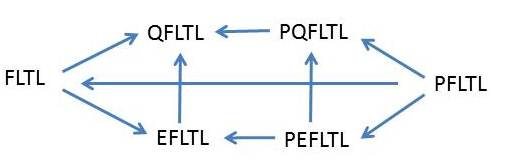
\includegraphics[height=1.5in,width=3in]{FIRST.jpg}
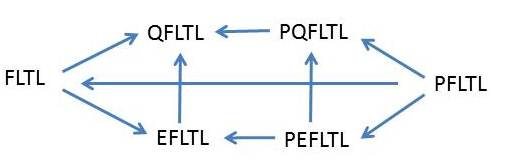
\includegraphics[width=3in]{FIRST.jpg}
\caption{\label{fsfr} An arrow from A to B means that logic  B is more expressive than A}
\end{center}
\end{figure}
}

\section{RV for Past-Time
First-Order  LTL and its Extension}
\label{EPLTLRV}

Runtime verification of FLTL is performed on an
input that consists of {\em events} in the form of
tuples. In our notation, the input
consists of a sequence ${\cal R}[1] \, {\cal R}[2]  \ldots$,
which we earlier identified with states, where each
${\cal R}[i]$ consists of the relations in
${\cal R}$ with
the last parameter is restricted to  $i$. A typical use
of runtime verification restricts the
events (tuples from the relations in ${\cal R}$) for
each state to a finite number, and often even to a single event.
The RV algorithm will also make
use of sets of assignments over a set of variables for satisfying a subformula at
some state, corresponding to $\old$ and $\current$, which had Boolean values in the 
algorithm for propositional LTL in Section~\ref{LTLruntime}.

\ignore{
\klaus{In the text above there are some imprecisions, such as
(1) ``tuples of relations'' - relations are sets of tuples, we don't have tuples of relations. 
(2) ``${\cal R}[i]$ consists of some relations'': it is a set of
relations (I think).
(3) ``to have, per each state just some finite tuples'': tuples are finite. You mean: to contain a finite set of tuples?
(4) what is the story about a set of assignments also being a relation? Needed?
}}

%\subsubsection{Syntax}

\ignore{
\klaus{Below: (\ref{EFLTL}) was not a EPFLTL form of specification.}}


\iffalse
, restricted to the past operators. We now present the definition of EPFLTL, the final main logic proposed in this paper. 
The syntax is as follows:


\[ 
\psi \mathrm{\ where\ } r_j ( x_j) := 
\varphi_j (x_j) : j \in \{ 1 , \ldots , n \}
\]
\begin{center}
$\varphi ::= \true  \; | \;
    p ( a ) \; | \;
    p ( x ) \; | \;
    ( \varphi \wedge \varphi ) \;  |   \;
   \neg \varphi \; | \;
    \ominus \varphi \; | \;
    ( \varphi  \; \since  \; \varphi ) \; | \;
    \exists x \; \varphi$
\end{center}

\klaus{Note that $\psi$ above is not defined as a syntactic category. It should really be $\varphi$. Likewise in other parts of the paper. Perhaps too big a change now? Also, there should be
a greek letter for a specification. E.g.:

\[ 
\pi ::= \varphi \mathrm{\ where\ } r_j ( x_j) := 
\varphi_j (x_j) : j \in \{ 1 , \ldots , n \}
\]
\[
\varphi ::= ...
\]}
\fi

\iffalse
\noindent {\bf Set Semantics.}
We now refine the semantics of the logic. Under the new definition, 
$I [ \varphi , \sigma, i ]$ is a function that returns
a set of assignments such that $\gamma \in I [ \varphi , \sigma, i ]$ 
iff $( \gamma , \sigma , i ) \models \varphi$.
This redefinition will later lead to a simple implementation 
using BDDs, where each set of assignments will be represented
as a BDD, and the Boolean operators will correspond directly 
to Boolean operators on BDDs.

In order to deal with subformulas with different sets of free
variables (hence, different domains for assignments), 
we apply a projection and an extension operator to assignments
over a subset of the variables. Let $\Gamma$ be
a set of assignments over the variables $W$, and
$U \subseteq W$.
Then $\proj ( \Gamma , U )$ (for ``projecting {\em out}'' or  ``hiding''
the variables $U$)
is the largest set of assignments over 
$W \setminus U$, 
each agreeing with some
assignment of $\Gamma$ on all the variables in $W \setminus U$.
Let $U \cap W = \emptyset$, then
$\ext ( \Gamma , U )$ is the largest set of assignments
over $W \cup U$, where each such assignment agrees 
with some assignment in $\Gamma$ on the
values assigned to the variables $W$. 
This means that we extend $\Gamma$ by
adding arbitrary values to the variables in $U$ from their domains.
Then $\proj ( \ext ( \Gamma , U ) , U ) = \Gamma$ holds.
We define the union and intersection operators on sets of
assignments, even if they are defined over non identical
sets of variables. 
In this case, the assignments are extended
over the union of the variables. Thus, if $\Gamma$ is a
set of assignments over $W$ and $\Gamma'$ is
a set of assignments over $W'$, then
$\Gamma \; \bigcup \;  \Gamma'$ is defined as $\ext (\Gamma , W' \setminus W ) \cup
\ext ( \Gamma' , W \setminus W' )$ and
$\Gamma \; \bigcap \; \Gamma'$ is $\ext (\Gamma , W' \setminus W ) \cap
\ext ( \Gamma' , W \setminus W' )$.  Hence, both are defined
over the set of variables $W \cup W'$.



%We define $\mathbf{F}$ and $\mathbf{T}$ as special constants
%in order to interpret formulas without free variables.
%They are the complement of each other.
%When combined with set operators (complementation, union, intersection),
%$\mathbf{F}$ behaves as the empty set, hence is idempotent to
%union. Accordingly, $\mathbf{T}$ is idempotent to intersection.


%\klaus{One may of course ask whether the following section on the 
%set semantics is needed. Maybe it is needed, since we probably need a semantics. Something to consider.}
\fi

\subsubsection{Set Semantics.}

The RV algorithm for
(E)PLTL, presented in~Section \ref{LTLruntime}
calculates
$\current ( \eta )$, for $\eta$ a
subformula of the monitored property, to be the
truth value of $\varphi$ over the
prefix inspected by the RV algorithm so far. For (E)PFLTL,
$\current (\eta )$ consists of the
sets of assignments (in the form of relations
over the free variables in the subformula),
rather than Boolean variables.


We redefine the semantics for EPFLTL in
equivalent way, which will be more directly related to the calculation of values
in $\current$ by the
RV algorithm that will be presented below. 
Under the  {\em set semantics}
(introduced in~\cite{HPU} for PFLTL, and extended here for EPFLTL),
$I [ \varphi , \sigma, i ]$ is a function that returns
a set of assignments such that $\gamma \in I [ \varphi , \sigma, i ]$ 
iff $( \gamma , \sigma , i ) \models \varphi$.

We present here only two simple cases of the set semantics. The full set semantics appears in the appendix. 
\begin{itemize}
\item $I [ ( \varphi \wedge \psi ) , \sigma , i ] = 
I [ \varphi , {\cal R} , i ] \;  \bigcap \; I [ \psi , \sigma , i ]$.
\item $I [ ( \varphi \; \since \; \psi ) , {\cal R} , i ] = 
I [ \psi , {\cal R}, i ] \; \bigcup \;
( I [ \varphi , {\cal R} , i ] \ \bigcap \ 
I [ (\varphi \since \psi ) , {\cal R} , i - 1 ] )$.
\end{itemize}



\subsubsection{Runtime verification algorithm for PFLTL.}

We start by describing an algorithm for monitoring 
PFLTL properties, first presented in~\cite{HPU} and implemented
in the tool~\dejavu. 
We enumerate data values appearing in
monitored events, as soon as we first see them. We
represent relations over the Boolean
encodings of these enumeration, rather than over the data values themselves. A hash function is used to connect the data values to their enumerations to maintain consistency
between these two representations.
The relations are
represented as BDDs~\cite{Bryant}. 
For example, if the runtime verifier sees the input 
events 
$\mathit{open}(\text{``a''})$, 
$\mathit{open}(\text{``b''})$, 
$\mathit{open}(\text{``c''})$, 
it will encode them as
$000$, $001$ and $010$ (say, we use 3 bits $b_0$, $b_1$ and $b_2$
to represent each enumeration, with $b_2$ being the most significant bit).
%
A Boolean representation of the {\em set} of values 
$\{\text{``a''},\text{``b''}\} $ would be equivalent to a Boolean function $(\neg b_1 \wedge \neg b_2)$ that returns 1 for $000$ and $001$ (the value
of $b_0$ can be arbitrary).

%

Since we want to be able to deal with infinite domains
(where only a finite number of elements may appear in a given observed prefix) and maintain the ability to perform
complementation, unused enumerations represent the
values that have not been seen and their relations
to all other values. 
%The algorithm maintains that these unseen values are correctly represented, as shown in~\cite{HPU}. 
In fact, it is sufficient to have just one enumeration representing these values per each variable of the LTL formula. 
%However, it is important to guarantee that at least one such enumeration exists. 
We guarantee that at least one such enumeration exists by preserving for that purpose the enumeration $11\ldots11$.
%, i.e., the highest Boolean representation,
%to represent values not yet seen.
We present here only the basic algorithm. For versions that
allow extending the number of bits used for enumerations and garbage collection of enumerations, consult~\cite{HP}.

\iffalse
Our preferred representation of a set of values (assignments) is as an Ordered Binary Decision
Diagram (OBDD, although we write simply BDD)~\cite{Bryant}.
A BDD~\cite{Bryant} is essentially a compact representation 
of a Boolean tree, where compaction glues together isomorphic subtrees. Each non-leaf node is labeled with one of the
Boolean variables $b_0,\ldots,b_{k-1}$ (where $k$ is the number of bits used to represent the values of a variable). A non-leaf node $b_i$ 
is the source of two 
arrows leading to other nodes, representing respectively that the node has the value 0 (false) or 1 (true).
%A dotted-line arrow represents that $b_i$ has the Boolean value $0$, while a thick-line 
%arrow represents that it has the value $1$. 
The nodes in the DAG have the
same order along all paths from the root. However, some of the nodes may be
absent along some paths, when the result of the Boolean function does not 
depend on the value of the corresponding Boolean variable. Each path leads 
to a leaf node that is marked by either a $0$ or a $1$, representing the 
Boolean value returned by the function for the Boolean values on the path.
\fi

The use of BDDs can be replaced by other representations that
can compactly and efficiently represent sets of values (e.g., ZDDs), and to which one can apply set operations like complementation, intersection, union (which are simply negation, conjunction and disjunction
in BDDs) and projection (for the quantification).
The marriage of BDDs and Boolean enumeration is in particular
efficient, since collections of adjacent Boolean enumerations tend to compact well.



\iffalse %%%%%
The definition of the {\em since} operator $S$ can be rewritten in a standard
way such that it refers only to the positions $i$ and $i-1$ in
the sequence $\sigma$. 
This is based on the
fact that according to the semantics of {\em since},
$(\varphi \, \since \, \psi) = ( \psi \vee (\varphi \wedge \ominus 
(\varphi \, \since \, \psi )))$.
This will serve in the
implementation to work with only two versions of
the sets of assignments, for the current and previous state:

\begin{itemize}
\item $( \gamma , \sigma , i ) \models ( \varphi \, \since \, \psi )$ if
$( \gamma |_{\vars ( \psi )} , \sigma , i ) \models \psi$ or $i>1$,
$( \gamma |_{\vars ( \varphi )} , \sigma , i ) \models \varphi$, and 
$( \gamma , \sigma , i-1 ) \models ( \varphi \, \since \, \psi )$.
\end{itemize}
\fi %%%%%
 
%The rest of the operators are defined as follows:
%$\false = \neg \true$, $\forall x \; \varphi = \neg \exists x \neg \varphi$,
%$(\varphi \vee \psi) = \neg ( \neg \varphi \wedge \neg \psi )$.
%We can also define the following useful operators:
%$P \varphi = (\true \, \since \, \varphi)$ (for ``previously''),
%$( \varphi \, R \, \psi ) = \neg ( \neg \varphi \, \since \, \neg \psi )$ 
%(the dual of the Since operator), and
%$H \varphi = ( \false \, R \, \varphi )$ (for ``always in the past'').

%\noindent {\bf Set Semantics.}
%It helps to represent the algorithm to 
%redefine the semantics of
%the logic in terms of sets of assignments satisfying a formula.
%Then $I [ \varphi , \sigma, i ]$ is a function that returns
%a set of assignments such that $\gamma \in I [ \varphi , \sigma, i ]$ 
%%Then a BDD for a set containing the values ``de'' and ``af''
%%(2nd and 3rd values)
%will return $1$ for $01$ and $10$. If the Boolean function is over
%$b_0$ (for most significant bit) and $b_1$ (for least significant), 
%then this is the Boolean function 
%$(\neg b_0 \wedge b_1) \vee (b_0 \wedge \neg b_1)$.

Given some ground predicate $p ( a )$, observed in the monitored execution, 
matching with $p ( x )$ in the monitored property,
let $\lookup ( x, a )$ be the enumeration of $a$ (a lookup in the hash table). If this
is $a$'s first occurrence, then it will be assigned a new enumeration.
Otherwise, $\lookup$ returns the enumeration that $a$ received before. We can use a counter, for each variable $x$, counting the number of different values appearing so far for $x$. When a new value appears, this counter is incremented, and the value is converted to
a Boolean representation. 
%Enumerations that were not yet used represent
%the values not seen yet. 
%In particular, we always leave at least
%one enumeration, $11\ldots 11$, for this purpose.
%In the next section we introduce data reclaiming, which allows 
%reusing enumerations for values that no longer affect the checked 
%property. 
%This involves a more
%complicated enumeration mechanism.


The function $\bddset (x, A)$ returns
a BDD that represents the set of assignments where $x$ is mapped to 
(the enumeration of) $v$ for
$v \in A$. This BDD is independent
of the values assigned to any variable
other than $x$, i.e., they can have any value.
For example, assume that we use the three Boolean variables (bits) $x_0$, $x_1$ and $x_2$
for representing enumerations over $x$ (with $x_0$ being the least significant bit), and
assume that $A = \{ a , b \}$, 
$\lookup ( x, a ) = 000$, and $\lookup ( x , b ) = 001$.
Then $\bddset ( x , A )$ is a BDD representation of the Boolean function 
$(\neg x_1 \wedge \neg x_2)$. 
%But the BDD function will be independent of the values of Boolean variables
%representing other variables.
%Notice that $p ( x )$ is
%equivalent, and is represented as $\exists y \, \exists z \, p ( x )$
%when the variables used in the formula are $x$, $y$ and $z$.

Intersection and union of sets of assignments are translated simply
to conjunction and disjunction of their BDD representation,
respectively, and complementation
becomes BDD negation. We will denote
the Boolean BDD operators as $\bddwedge$, $\bddvee$ and $\bddneg$.
To implement the existential (universal, respectively) operators, 
%as in the interpretation of $\exists x \; \varphi$, 
we use the BDD existential (universal, respectively) operators over
the Boolean variables that represent (the enumerations of) the values of $x$. 
%Thus, $x$ is translated into
%is represented using the Boolean variables $x_1$, $x_1, \ldots x_{k}$ into 
Thus, if $B_{\varphi}$ is the BDD representing
the assignments satisfying $\varphi$ in
the current state of the monitor, then 
$\bddexists (\langle x_0,\ldots,x_{k-1} \rangle, B_{\varphi})$
is the BDD that represents the assignments satisfying $\exists x \; \varphi$ in the current
state.
Finally, $\bfalse$ and $\btrue$  are the BDDs that return always
$0$ or $1$, respectively.

%The case where the number of bits used to represent values for
%some domains is eventually insufficient is dealt with by
%expanding the number of bits for the BDD. This will be explained later,
%but is much harder to implement, and may require a lot of overhead
%to update the BDDs while online computation is monitored. This
%may be unnecessarily, as we can assign a large number of bits
%a priory, where these bits represent a set of values that is
%exponentially larger.

\iffalse
The algorithm shown below uses two vectors (arrays) of values indexed by subformulas: 
$\old$ for the state before that event, and
$\current$ for the current
state (after the last seen event).
While in the propositional case, in Section~\ref{LTLruntime}, the vectors contain Boolean values, here
they contain BDDs. The temporal relations,
restricted to each state, are
represented also as BDDs.
The algorithm follows.
\fi

\begin{enumerate}
\item Initially, for each subformula $\varphi$ of $\eta$,
%$B ( \varphi , \current ) = \bfalse$.
$\current ( \varphi ) := \bfalse$.
\item Observe a new state (as a set of ground predicates) $s_i$ as input. 
\item Let $\old := \current$.
\item Make the following updates for each subformula. If $\varphi$ is
      a subformula of $\psi$ then $\current ( \varphi )$ is updated before 
      $\current ( \psi )$.
\begin{itemize}
  \item $\current ( \true ) := \btrue$.
  \item $\current ( p_k ( a ) )$ := if $R_k [ i ] ( a )$ then
  $\btrue$ else $\bfalse$.
  \item $\current ( p_k ( x ) )$ :=
     $\bddset ( x ,  \{ a \ | \ R_k[i] ( a  ) \} )$.
  \item $\current ( ( \varphi \wedge \psi ) ) := 
  \bddwedge ( \current ( \varphi ) , \current ( \psi ))$.
  \item $\current ( \neg \varphi  ) := \bddneg ( \current ( \varphi ))$.
  \item $\current ( ( \varphi\ \since\ \psi ) ) :=  
  \bddvee ( \current ( \psi  ) , \bddwedge ( \current ( \varphi ) ,
      \old ( ( \varphi \ \since \ \psi ))))$.
%DAP: I removed the \; around \since, since it penetrated the 2nd column!
  \item $\current ( \ominus \; \varphi ) := \old ( \varphi )$.
  \item $\current ( \exists x \; \varphi ) := 
  \bddexists (\langle x_0,\ldots,x_{k-1} \rangle, \current ( \varphi ))$.
\end{itemize}
\item If $\current (\eta) = \false$ then
report a violation, otherwise goto step~2.
\end{enumerate}

\subsubsection{Runtime verification algorithm for EPFLTL}

We extend now the algorithm to capture EPFLTL.
The auxiliary relations $r_j$ extend the model, and we need to keep 
BDDs representing $\current ( r_j )$ and
$\old (r_j)$ for each relation $r_j$. We also need to calculate the 
subformulas $\varphi_i$ that appear in
a specification, as part of the runtime verification,
as per the above FPLTL algorithm. One subtle point is that the auxiliary 
relations $r_j$ may be defined in a rule with respect to
a variable $x_j$ (as $r_j (x_j ):= \varphi_j (x_j)$ (this can be generalized 
to any number of variables), but $r_j$ can be used
as a subformula with other parameters in other rules or in the statement e.g., 
as $r_j ( y )$. This can be resolved by a BDD renaming function 
$\rename ( r_j (x_j ) , y)$.


We then have to add
following updates to step~4 of the above algorithm, when performing runtime verification of
$\psi$. 

\noindent \begin{description}
\item For each rule 
$r_j ( x_j ) := \varphi_j ( x_j )$:
\item{\ \ }  calculate $\current ( \varphi_j )$;
\item{\ \ }  $\current ( r_j )  := \current (\varphi_j)$;
\item{\ \ } $\current ( r_j ( y ) )$ := $\rename ( r_j(x_j) ,  y )$;
\item{\ \ } $\current ( r_j ( a ) )$ := if $\current ( r_j ) ( a )$
then $\btrue$ else $\bfalse$
\end{description}

%\klaus{Above: $\current ( r_j ) ( a )$ has not been defined I think.}

\noindent
As in the propositional case, the evaluation order cannot be
simply top down or bottom up, since relations can appear
both on the left and the right of a definition
such as $r ( x ) := p ( x ) \vee \ominus r ( x )$. For that,
we need to use the {\em mixed} evaluation order, described in Section~\ref{LTLruntime}.













